% !TEX root = main.tex

%-------------------------------------------------
\section{Location-scale models}

We seek to identify classes of parameters, in particular \emph{location parameters} and \emph{scale parameters}. 

We can think of a parameter as a \emph{function} of the CDF (or PDF/PMF) of a random variable: we call these \emph{functionals}\footnote{The term \textit{functional} is a generic term used for a function that maps functions to scalar values.}. 
%For example, the mean of $X$ can be expressed by the \emph{mean functional},
%\[
%T(F) = \int_{-\infty}^{\infty} xf(x)\,dx.
%\]
%Likewise, the median of $X$ can be expressed as the \emph{median functional},
%\[
%T(F) = F_X^{-1}(1/2).
%\]
For example,
\[\begin{array}{lll}
T(F_X) & = \displaystyle\int_{-\infty}^{\infty} xf_X(x)\,dx	& \qquad\text{is the \emph{mean functional},} \\[2ex]
T(F_X) & = F_X^{-1}(1/2)	& \qquad\text{is the \emph{median functional}.}
\end{array}
\]

% remark: induced estimators
\begin{remark}
The empirical CDF $\hat{F}_X$ is itself a CDF so we can apply the functional $T$ to $\hat{F}_X$:
\bit
\it $T(\hat{F}_X)$ is called the \emph{induced estimator} of $T(F_X)$. 
\eit
For example,
\bit
\it if $T$ is the mean functional, $T(\hat{F}_X)$ is the sample mean;
\it if $T$ is the median functional, $T(\hat{F}_X)$ is the sample median.
\eit
\end{remark}

% defn: location and scale functionals
\begin{definition}
\ben
\it $T$ is said to be a \emph{location functional} if 
\[
T(F_{a+bX}) = a + bT(F_X) \quad\text{for all $a,b\in\R$.}
\]
\it $T$ is said to be a \emph{scale functional} if 
\[
T(F_{a+bX}) = bT(F_X) \quad\text{for all $b>0$.}
\]
\een
\end{definition}

% example: mean and standard deviation
\begin{example}
\ben
\it Show that the mean is a location functional.
\it Show that the standard deviation is a scale functional.
\een
\begin{solution}
Let $Y=a+bX$. By the linearity of expectation, the mean functional $T(F_X) = \expe(X)$ sastifies
\[
T(F_{a+bX})= \expe(a+bX) = a+b\expe(X) = a + bT(F_X),
\]
and the standard deviation functional $T(F_X) = \sqrt{\var(X)}$ sastifies
\[
T(F_{a+bX}) = \sqrt{\var(a+bX)} = \sqrt{b^2\var(X)} = b\sqrt{\var(X)} = bT(F_X)
\]
as required.
\end{solution}
\end{example}

%% remark: induced estimators
%\begin{remark}
%Consider the empirical CDF of $X$, 
%\[
%\hat{F}_n(x) = \frac{1}{n}\sum_{i=1}^n I(X_i\leq x) 
%\]
%
%Because $\hat{F}_n$ is itself a CDF, we can apply the functional $T$ to $\hat{F}_n)$.
%\bit
%\it $T(\hat{F}_n)$ is called the \emph{induced estimator} of $T(F)$. 
%\it
%
%For example,
%\bit
%\it if $T(F)$ is the mean functional, $T(\hat{F}_n)$ is the sample mean;
%\it if $T(F)$ is the median functional, $T(\hat{F}_n)$ is the sample median.
%\eit
%\end{remark}
%-----------------------------
%\subsection{Location-scale models}
%
%Let $X$ be a random variable, let $T(F_X)$ be a location functional and consider the random variable $Z = X - T(F_X)$. Because $T$ is a location functional, $T(F_Z)=0$ and the PDF of $X$ can be written as 
%\[
%f_X(x) = f_Z(x-T(F_X)).
%\]
%
%% location model
%\begin{definition}[Location models]
%A statistical model for the distribution of $X$ is called a \emph{location model} with location functional $\theta_X = T(F_X)$ if 
%\[
%X = T(F_X) + Z
%\]
%where $Z$ is a random variable with $T(F_Z)=0$.
%\end{definition}
%
%Simpler version:
%\begin{definition}
%Let $\mathcal{M}=\{F(x;\theta):\theta\in\Theta\}$ be a statistical model for the distribution of $X$.
%\ben
%\it $\mathcal{M}$ is called a \emph{location model} if for every $F\in\mathcal{M}$ and $a\in\R$, the CDF $G(x)=F(a+x)$ also belongs to $\mathcal{M}$.
%\it $\mathcal{M}$ is called a \emph{scale model} if for every $F\in\mathcal{M}$ and $b\in\R$ with $b>0$, the CDF $G(x)=F(bx)$ also belongs to $\mathcal{M}$..
%\it $\mathcal{M}$ is called a \emph{location-scale model} if for every $F\in\mathcal{M}$ and $a,b\in\R$ with $b>0$, the CDF $G(x)=F(a+bx)$ also belong $\mathcal{M}$.
%\een
%\end{definition}

% location and location-scale models
\begin{definition}
A statistical model $\mathcal{M}$ is called a
%\ben
%\it \emph{location model} if for every $F\in\mathcal{M}$ and $a\in\R$, the CDF $G(x)=F(a+x)$ also belongs to $\mathcal{M}$. 
%\it \emph{location-scale model} if for every $F\in\mathcal{M}$ and $a,b\in\R$ with $b>0$, the CDF $G(x)=F(a+bx)$ also belongs $\mathcal{M}$.
%\een
\ben
\it \emph{location model} if $F(a+x)\in\mathcal{M}$ whenever $F\in\mathcal{M}$ and $a\in\R$.
\it \emph{location-scale model} if $F(a+bx)\in\mathcal{M}$ whenever $F\in\mathcal{M}$ and $a,b\in\R$ with $b>0$.
\een
\end{definition}

\begin{example}
Show that the family of uniform distributions $\mathcal{M}=\left\{\displaystyle\frac{x-L}{R-L}:L,R\in\R, L<R\right\}$ is a location-scale model.
\begin{solution}
For $Y=a+bX$ where $X\sim\text{Uniform}[L,R]$,
\[
F_Y(y) = \prob(Y\leq y) = \prob\left(X\leq\frac{y-a}{b}\right) 
	= \frac{(y-a/b)-L}{R-L} 
	= \frac{y - (a+bL)}{(a+bR)-(a+bL)}.
\]
Hence $Y\sim\text{Uniform}[a+bL, a+bR]$ so $F_Y\in\mathcal{M}$.
\end{solution}
\end{example}

%\begin{example}
%Show that the family of normal distributions $\mathcal{M}=\{f(x;\mu,\sigma^2):\mu\in\R,\sigma^2\in\R^+\}$ is a location-scale model.
%\begin{solution}
%For $Y=a+bX$ where $X\sim N(\mu,\sigma^2)$,
%\[
%Y \sim N(a+b\mu, b^2\sigma^2)
%\]
%so $F_Y\in\mathcal{M}$.
%\end{solution}
%\end{example}

%-----------------------------
\subsection{Q-Q plots}
Let $\mathcal{M}$ be a location-scale model and let $Z$ be a random variable whose CDF $F_Z\in\mathcal{M}$ is known. Suppose we have another random variable $X$ whose CDF $F_X$ is unknown, and that we wish to test whether $F_X\in\mathcal{M}$. 

%Let $Z$ be a random variable whose CDF $F_Z$ is known, and suppose that $F_Z\in\mathcal{M}$ where $\mathcal{M}$ is a location-scale model. Suppose we have another random variable $X$ whose CDF $F_X$ is unknown, and that we wish to test whether or not $F_X\in\mathcal{M}$. 

Because $\mathcal{M}$ is a location-scale model, if $F_X\in\mathcal{M}$ then
\[
X = a + bZ %\quad\text{for $a,b\in\R$ with $b>0$,}
\]
where $a$ and $b>0$ are unknown parameters. Since $b>0$ the CDF of $X$ satisfies
\[
F_X(x) = \prob(X\leq x) = \prob(a+bZ\leq y) = \prob\left(Z\leq\frac{x-a}{b}\right) = F_Z\left(\frac{x-a}{b}\right).
\]

Let $x_p$ and $z_p$ denote the $p$th quantiles of $X$ and $Z$ respectively (where $0<p<1$). Then
\bit
\it $z_p = F_Z^{-1}(p)$ is known
\it $x_p = a + bF_Z^{-1}(p)$ is unknown (because $a$ and $b$ are unknown).
\eit
If $F_X\in\mathcal{M}$ we have the linear relationship 
\[
x_p = a + b z_p.
\]

%\bigskip
The quantiles $x_p$ of $F_X$ are unknown, but they can be estimated by order statistics.
\bit
%\it Let $X_1,X_2,\ldots,X_n$ be a random sample from the distribution of $X$.
%\it Let $X_{(1)},X_{(2)},\ldots,X_{(n)}$ be the order statistics of $X_1,X_2,\ldots,X_n$.
%\it Let $X_1,X_2,\ldots,X_n$ be a random sample from the distribution of $X$.
\it Let $X_{(1)},X_{(2)},\ldots,X_{(n)}$ be the order statistics of a random sample from the distribution of $X$.
\it $X_{(k)}$ is a point estimator of the quantile $x_{p_k}$ where $p_k=k/(n+1)$.
\eit

\begin{definition}
A plot of the order statistics $X_{(k)}$ against the quantiles $z_{p_k}$ is called a \emph{Quantile-Quantile plot} (Q-Q plot).
\end{definition}

\bit
\it If $F_X\in\mathcal{M}$, the plot should be approximately linear.
\it The parameters $a$ and $b$ can be estimated by the intercept and gradient respectively.
\eit

% example: Q-Q plots
\begin{example}
To test whether a random sample $X_1,X_2,\ldots,X_n$ is from a Normal distribution, we plot the order statistics $X_{(k)}$ against the values $z_{p_k} = \Phi^{-1}\big[k/(n+1)\big]$ for $k=1,2,\ldots,n$ where $\Phi$ is the CDF of $N(0,1)$. If the points lie on (or near) a straight line, we might conclude that the $X_i$ are normally distributed (see Figure~\ref{fig:qq}). 
%\begin{minipage}{\linewidth}
%\begin{minipage}{0.45\linewidth}
%\resizebox{\linewidth}{!}{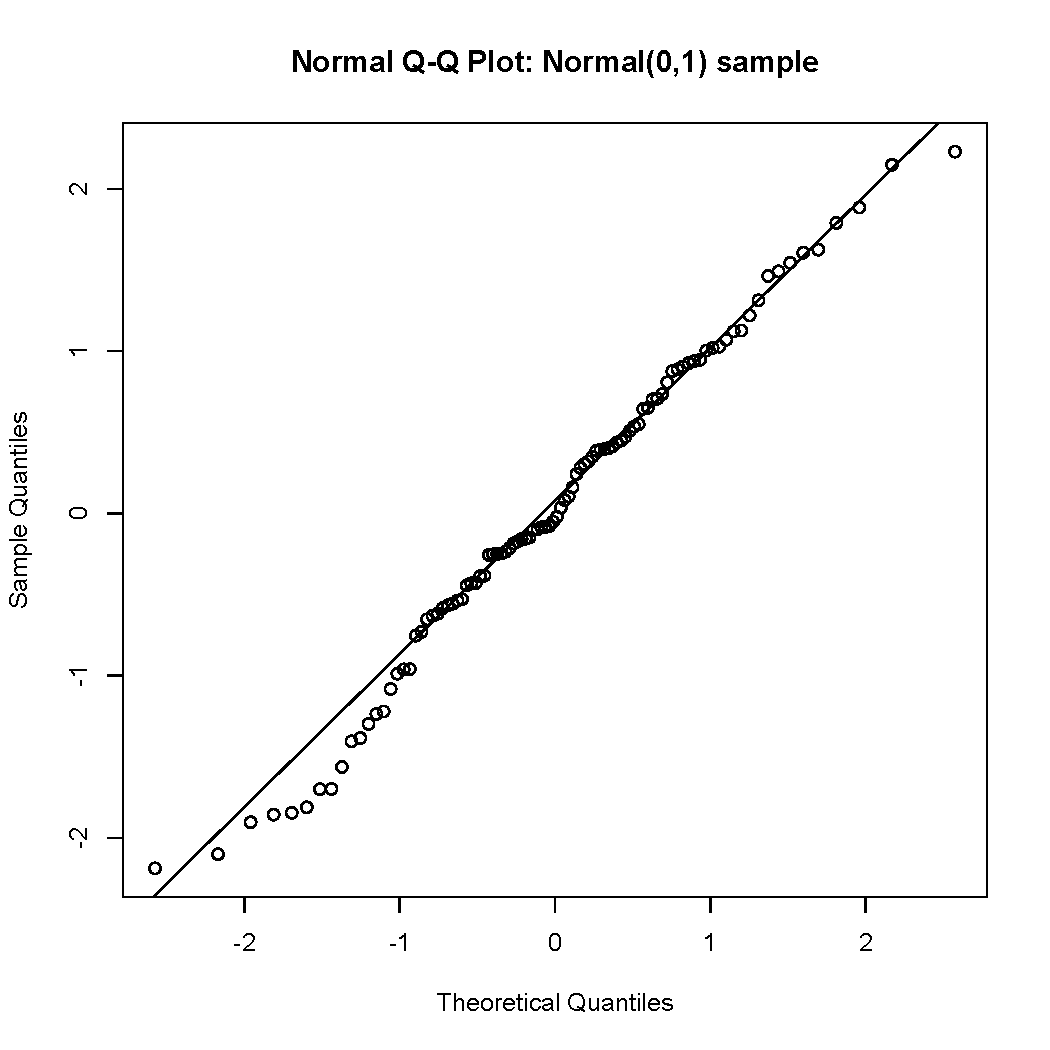
\includegraphics{nqqplot-normal}}
%\end{minipage}
%\hfill
%\begin{minipage}{0.45\linewidth}
%\resizebox{\linewidth}{!}{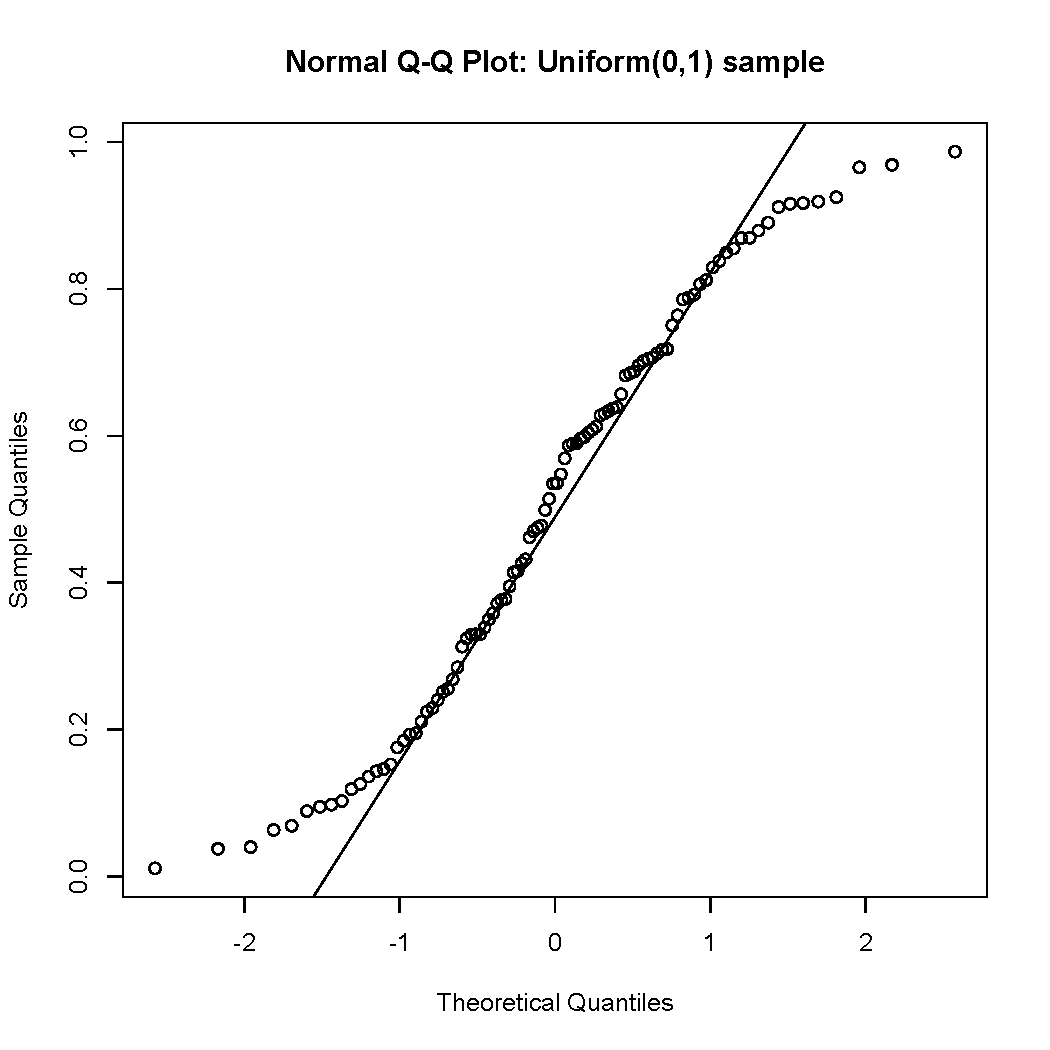
\includegraphics{nqqplot-uniform}}
%\end{minipage}
%\end{minipage}
\begin{figure}[ht]
\centering
\begin{tabular}{cc}
	\begin{subfigure}{0.45\textwidth}
	\resizebox{\linewidth}{!}{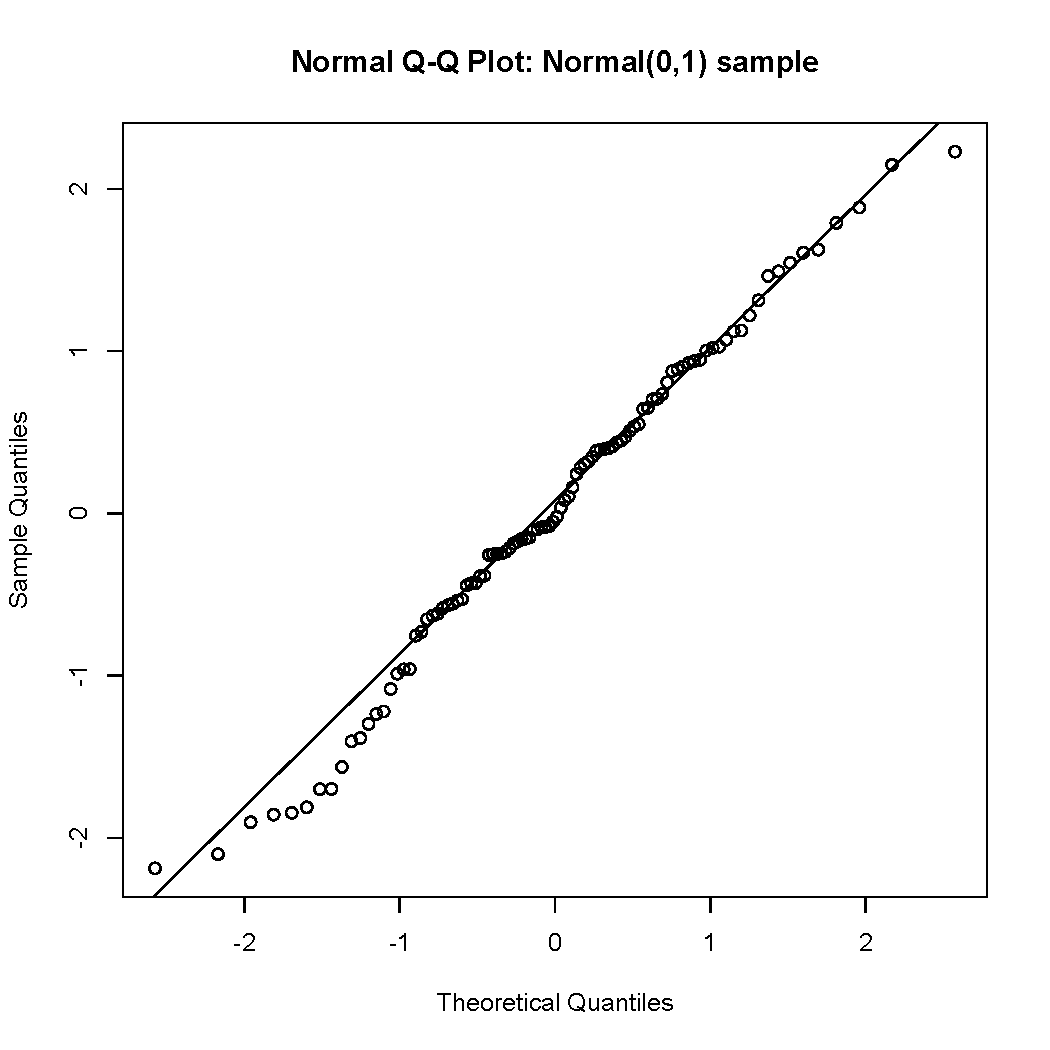
\includegraphics{nqqplot-normal}}
	\end{subfigure}
&
	\begin{subfigure}{0.45\textwidth}
	\resizebox{\linewidth}{!}{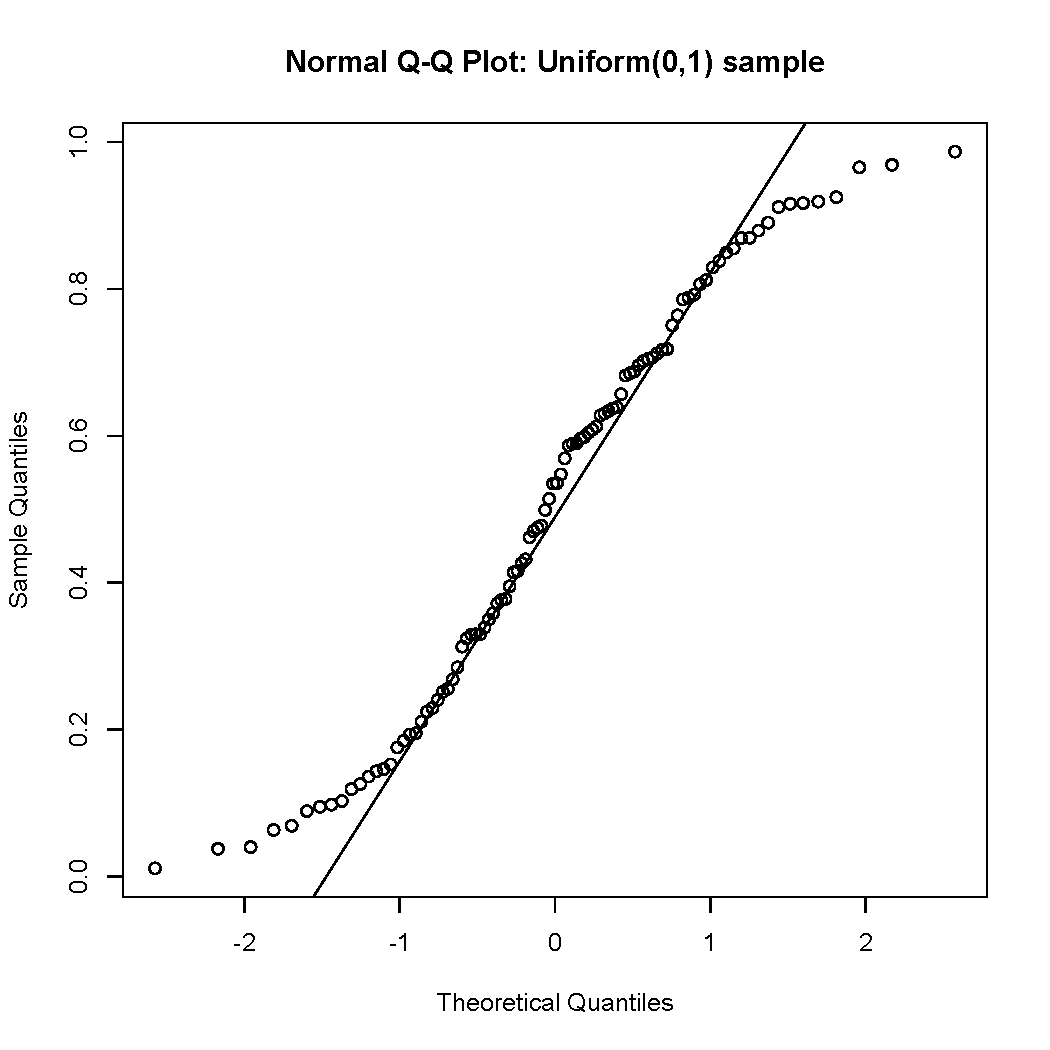
\includegraphics{nqqplot-uniform}}
	\end{subfigure}
\end{tabular}
\caption{Q-Q plots for testing normality.\label{fig:qq}}
\end{figure}

\end{example} 

% exercise (symmetric distributions)
\begin{exercise}
\begin{questions}
\question
Let $X$ be a random variable, let $F_X$ be its CDF and suppose that its distribution is symmetric about $a$.  Using the fact that $X-a$ and $-(X-a)$ have the same distribution, show that any location functional satisfies $T(F_X)=a$. 
\begin{answer}
Because $T$ is a location functional,
\[
T(F_{X-a}) = T(F_X)-a \qquad\text{and}\qquad T(F_{-(X-a)}) = -T(F_X)+a.
\]
Because $X-a$ and $-(X-a)$ have the same distribution, these are equal so $T(F_X)=a$, as required.
\end{answer}

\question %median and IQR
\begin{parts}
\part % median
Show that the median is a location functional.
\begin{answer}
Let $Y=a+bX$. Then
\[
F_{a+bX}(y) = \begin{cases}
	F_X\left(\frac{y-a}{b}\right)		& \text{ if $b>0$,} \\
	1 - F_X\left(\frac{y-a}{b}\right)	& \text{ if $b<0$.} 
\end{cases}
\]
Let $T(F_X)=F_X^{-1}(1/2)$ be the median functional. Then $F_X\big[T(F_X)\big] = 1/2$ so for $b>0$, 
\[
F_{a+bX}\big[a+bT(F_X)\big] = F_X\left[\frac{a+bT(F_X) - a}{b}\right] = F_X\big[T(F_X)\big] = 1/2,
\]
and for $b<0$, 
\[
F_{a+bX}\big[a+bT(F_X)\big] = 1 - F_X\left[\frac{a+bT(F_X) - a}{b}\right] = 1 - F_X\big[T(F_X)\big] = 1 - 1/2 = 1/2.
\]
In either case we have 
\[
T(F_{a+bX}) = F_{a+bX}^{-1}(1/2) = a+bT(F_X),
\]
so the median is a location functional, as required.
\end{answer}

\part % IQR
Show that the inter-quartile range is a scale functional.
\begin{answer}
Let $L(F_X) = F_X^{-1}(1/4)$ and $U(F_X)=F_X^{-1}(3/4)$ be the lower-quartile and upper-quartile functionals respectively. Then
\[
F_X\big[L(F_X)\big] = 1/4 \quad\text{and}\quad F_X\big[U(F_X)\big] = 3/4.
\]
For $b>0$, 
\begin{align*}
F_{a+bX}\big[a+bL(F_X)\big]
	& = F_X\left[\frac{a+bL(F_X) - a}{b}\right] = F_X\big[L(F_X)\big] = 1/4,\\
F_{a+bX}\big[a+bU(F_X)\big]
	& = F_X\left[\frac{a+bU(F_X) - a}{b}\right] = F_X\big[U(F_X)\big] = 3/4,\\
\end{align*}
Thus $L(F_{a+bX}) = F_{a+bX}^{-1}(1/4) = a+bL(F_X)$ and $U(F_{a+bX}) = F_{a+bX}^{-1}(3/4) = a+bU(F_X)$.

\bigskip
The inter-quartile range functional is $T(F_X)=U(F_X)-L(F_X)$, so
\[
T(F_{a+bX}) 
	= F_{a+bX}^{-1}(3/4) - F_{a+bX}^{-1}(1/4) 
	= \big[a+bU(F_X)\big] - \big[a + bL(F_X)\big]
	= b\big[U(F_X)-L(F_X)\big]
	= bT(F_X).
\]
Thus the inter-quartile range is a scale functional, as required.
\end{answer}
\end{parts}
\end{questions}
\end{exercise}


